\chapter{Evaluation}
\label{ch:evaluation}
This chapter presents the results of the data extraction from receipts, as well as the results of each module.

\section{API results}\label{sec:api-results}
The implementation of our API's are made as a MVP\@.
This means that there is little to no validation on the input and the output, which means it only really works when
you send in the correct input.

\subsection{.NET API}\label{subsec:.net-api}

When the right input is sent in, the API functions as expected.
The input is an ImageDTO that comes from a POST request sent from the React module.
The image data from the ImageDTO is then correctly converted to a base64 string, which is then sent to the ML API through a POST request.

The result of the POST requests to the ML API is converted in to a receipt object and returned to the React module
where it is correctly displayed in their respective fields.

\begin{figure}[h]
    \center{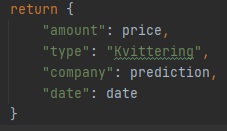
\includegraphics[width=0.8\textwidth]{Images/MLAPIreturnObject}}
    \caption{The result from the ML API}
    \label{fig:MLAPIreturnObject}
\end{figure}

\subsection{ML API}\label{subsec:ml-api}
The ML API takes in a base64 string from a POST request originating from the .NET API\@.
This string contains the image data, and is correctly converted to an image.
The image is then sent to the CNN and OCR\@.
From the CNN we get the company.
From the OCR we get the date, and a string, which is sent to Spacy and is used to get the price from the receipt.

The result of this is a json object with the corresponding data.
Shown in figure~\ref{fig:MLAPIreturnObject}

\section{CNN results}\label{sec:cnn-results}
Many different CNN models with slight variations in their parameters were trained and tested.
Initially, the models had a low prediction accuracy, predicting the correct category about one third of the time.
Tweaking was done to the model by adding dropout, data normalization and max pooling.
Prediction accuracy then went up to around 95\% for most models.

\begin{figure}[h]
    \center{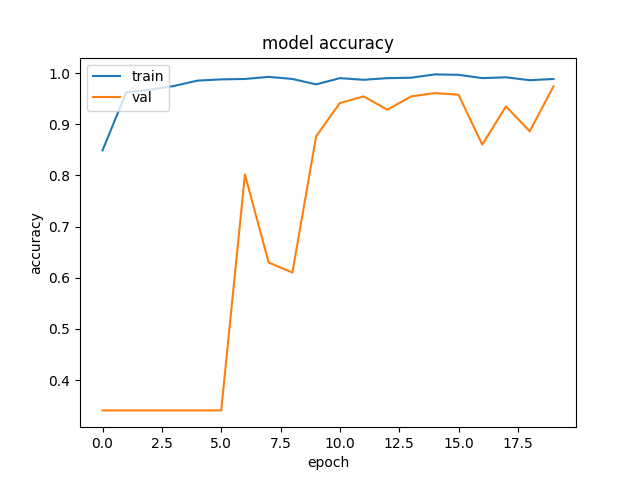
\includegraphics[width=1\textwidth]{Images/200modelaccuracy}}
    \caption{Training and validation accuracy for a model trained on 200x200 images}
    \label{fig:200modelaccuracy}
\end{figure}

Validation accuracy and loss are the two metrics we are using to determine the success of a model.
FIGURLINK and FIGURLINK shows how the model accuracy and loss are improving with each epoch of training.
A consistent theme when training our models was the validation accuracy and loss starting to radically improve between epoch 10 and 15.

\begin{figure}[h]
    \center{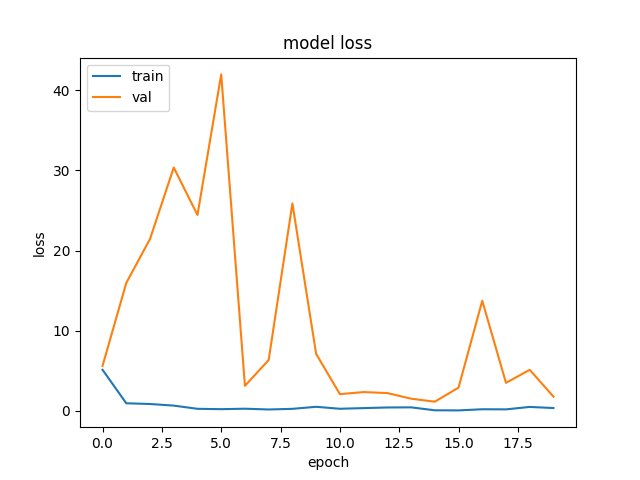
\includegraphics[width=1\textwidth]{Images/200modelloss}}
    \caption{Training and validation loss for a model trained on 200x200 images}
    \label{fig:200modelloss}
\end{figure}

\begin{figure}[h]
    \center{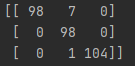
\includegraphics[width=1\textwidth]{Images/200confusion}}
    \caption{Confusion matrix for a model trained on 200x200 images}
    \label{fig:200confusion}
\end{figure}

A confusion matrix was also used to give some more insight into how the model was performing for each of the different categories it had been trained on.
FIGURLINK shows the confusion matrix generated from the same model as FIGURLINKACCURACY and FIGURLINKLOSS, using the same validation dataset.
The confusion matrix has three throws, one for each category of receipt the model has been trained to classify.
The diagonal of the matrix shows how many correct classifications the model made.
The rest of the fields shows how many incorrect classifications were made.
In FIGURLINK, we can see that for the second category, all the predictions made were correct.
We can also see that most of the incorrect predictions were done on the first category, with 7 of the 8 incorrect predictions taking place here.

When trying to do predictions on a single image, the results were more inconsistent.
Predictions were made using images from the same dataset that it was trained on, with varying success despite good accuracy from validation during training.
For example, model A and model B might both have gotten validation accuracies over 95\%.
When tested on single images model A would always predict that category 1 was category 2, while model B would predict the categories correctly.

\section{OCR results}\label{sec:ocr-results}
Since our OCR implementation uses pre-defined templates to de-skew images, the output of our CNN plays a big part in whether the OCR will be able to extract text from the images.
When the CNN does not accurately predict the correct category for an image, the OCR de-skew will use the wrong image template, and the result of this de-skew becomes an image that is unusable.
This can be seen in figures~\ref{fig:scuffedmatch2} and~\ref{fig:scuffedmatchresult}

\begin{figure}[h]
    \center{\includegraphics[width=1\textwidth]{Images/matchesscuffed2}}
    \caption{Input image (left) trying to match its content to the wrong image template (right)}
    \label{fig:scuffedmatch2}
\end{figure}

\begin{figure}[h]
    \center{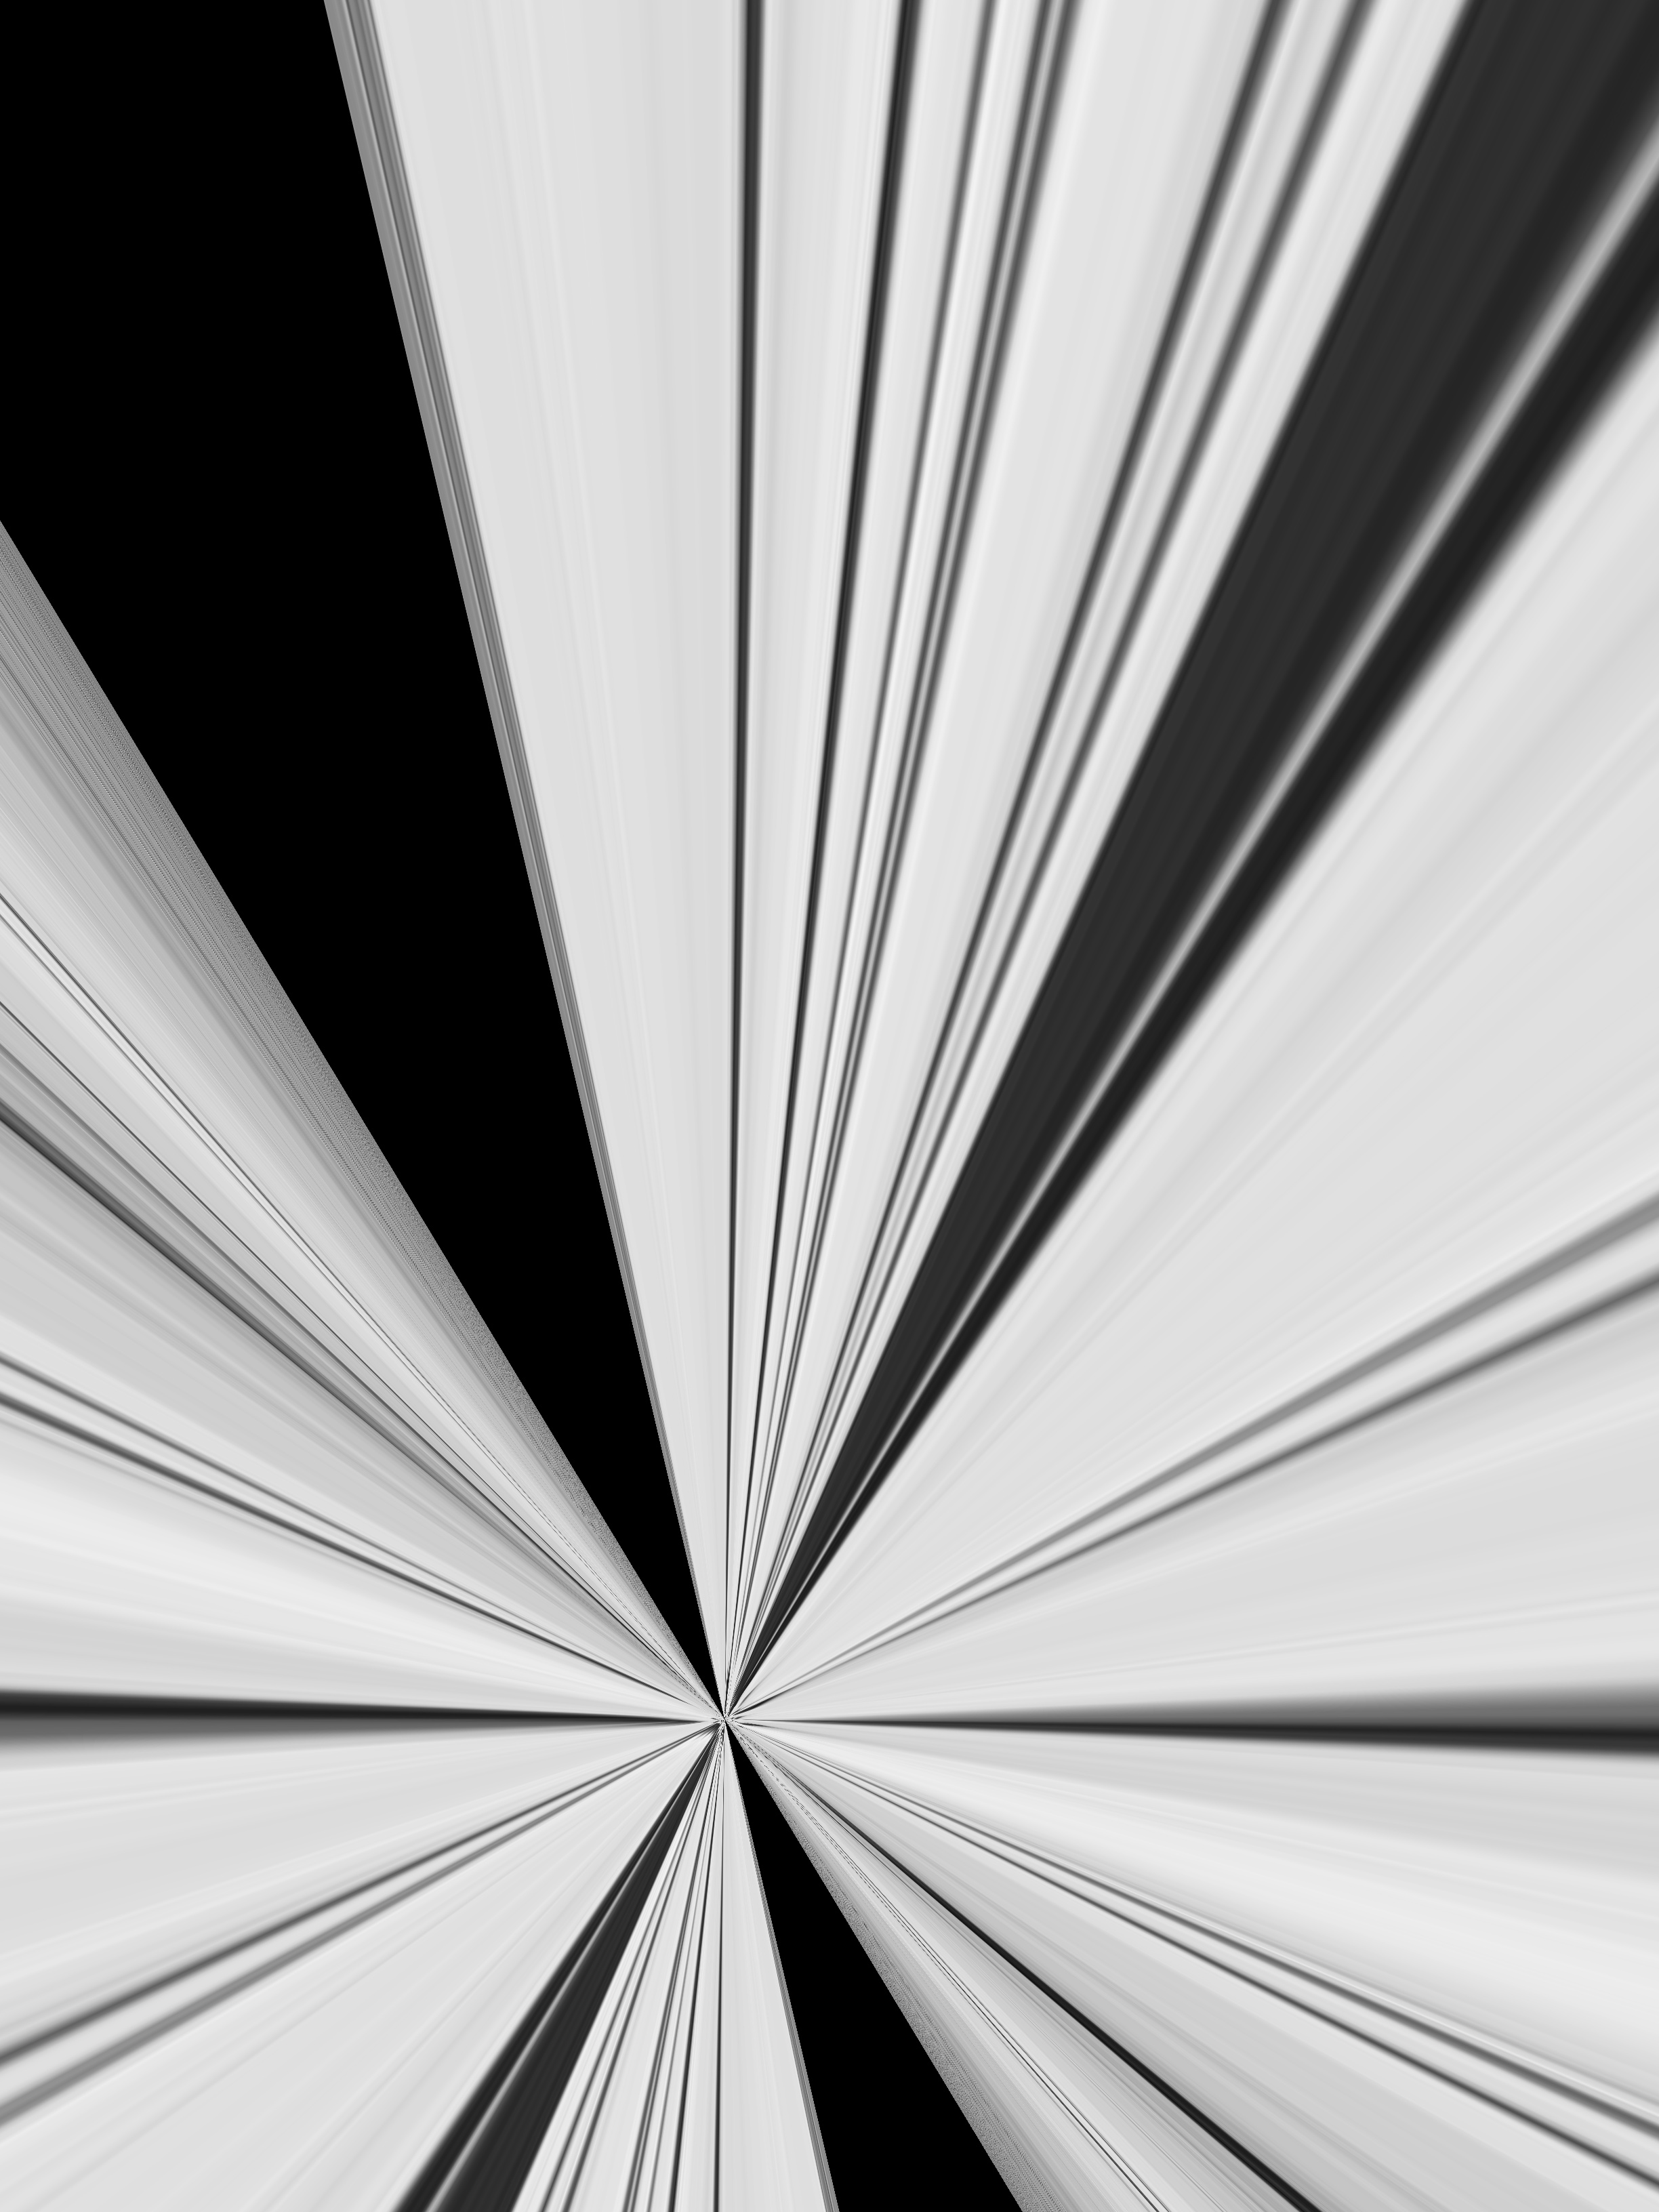
\includegraphics[width=1\textwidth]{Images/alignedscuffed}}
    \caption{Result of de-skewing when using the wrong image template}
    \label{fig:scuffedmatchresult}
\end{figure}

Because of this, the OCR module does not give any text output when the predicted category is not correct.
When isolating the OCR module from the other modules, or when the CNN predicts the correct category, the text output from our OCR module is mostly accurate.
However, small mistakes in the text extraction can lead to the wrong piece of data being extracted or not found at all.

\begin{figure}[h]
    \center{\includegraphics[width=1\textwidth]{Images/beforeafterpreprocess}}
    \caption{Before and after pre-processing}
    \label{fig:beforeaftepreprocess}
\end{figure}


Figure~\ref{fig:beforeaftepreprocess} shows the input image sent to the OCR on the left and the image after going
through pre-processing on the right.
Since the CNN made the correct prediction on what category of receipt this is, the de-skewing algorithm successfully straightened the image.
The figure also illustrates the binarization of the image, making the text easier to distinguish from the background.
An attempt to extract the text from the right-hand image is then being done.

\begin{figure}[h]
    \center{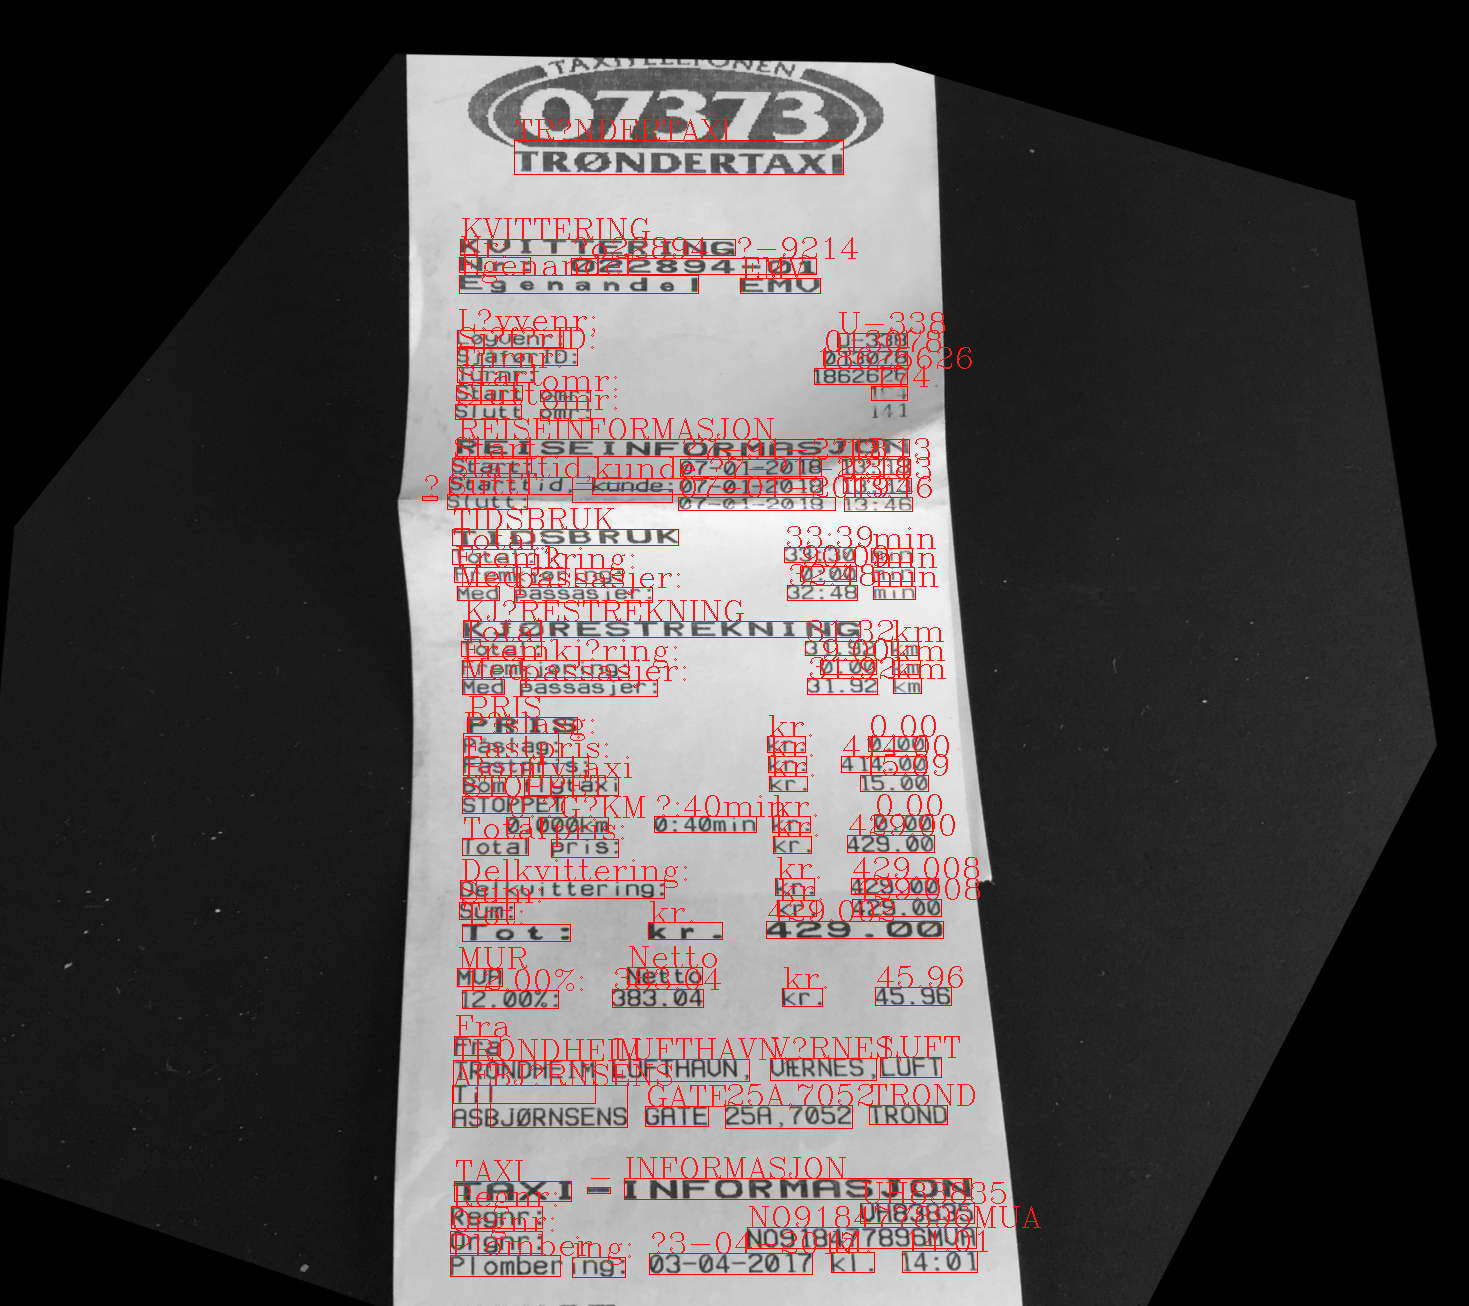
\includegraphics[width=1\textwidth]{Images/ocrtextboxes}}
    \caption{Extracted text in red, appearing over the place it has been extracted from}
    \label{fig:ocrtextboxes}
\end{figure}

Looking at figure~\ref{fig:ocrtextboxes}, the text seems to have been reasonably accurately extracted.
A date is then found using our regular expression for commonly used date formats.

\begin{figure}[h]
    \center{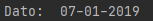
\includegraphics[width=1\textwidth]{Images/dateocr}}
    \caption{The date extracted from OCR output}
    \label{fig:dateocr}
\end{figure}

On further inspection, we can see that the date found in figure~\ref{fig:dateocr} does not match the date in
the image.
The date extracted from the OCR is from 2019, while the actual date should be 2018.
This means that the date that is given back to the API and back to the user, is not correct.
This example in particular highlights some issues with our implementation and will be discussed more in chapter 6.

The above example is a good indicator for what happens when the CNN correctly predicts the proper category, and when the image is readable by the OCR\@.
One of our categories of images were never readable by the OCR however.

\begin{figure}[h]
    \center{\includegraphics[width=1\textwidth]{Images/beforeafterflybuss}}
    \caption{Before and after pre-processing}
    \label{fig:beforeafterflybuss}
\end{figure}

\figurename{~\ref{fig:beforeafterflybuss}} shows the image as it is being sent from the user into our pipeline, and
after the OCR pre-processing.
The CNN made the correct prediction, as can be seen by the image not being rendered unusable by the de-skewing.

\begin{figure}[h]
    \center{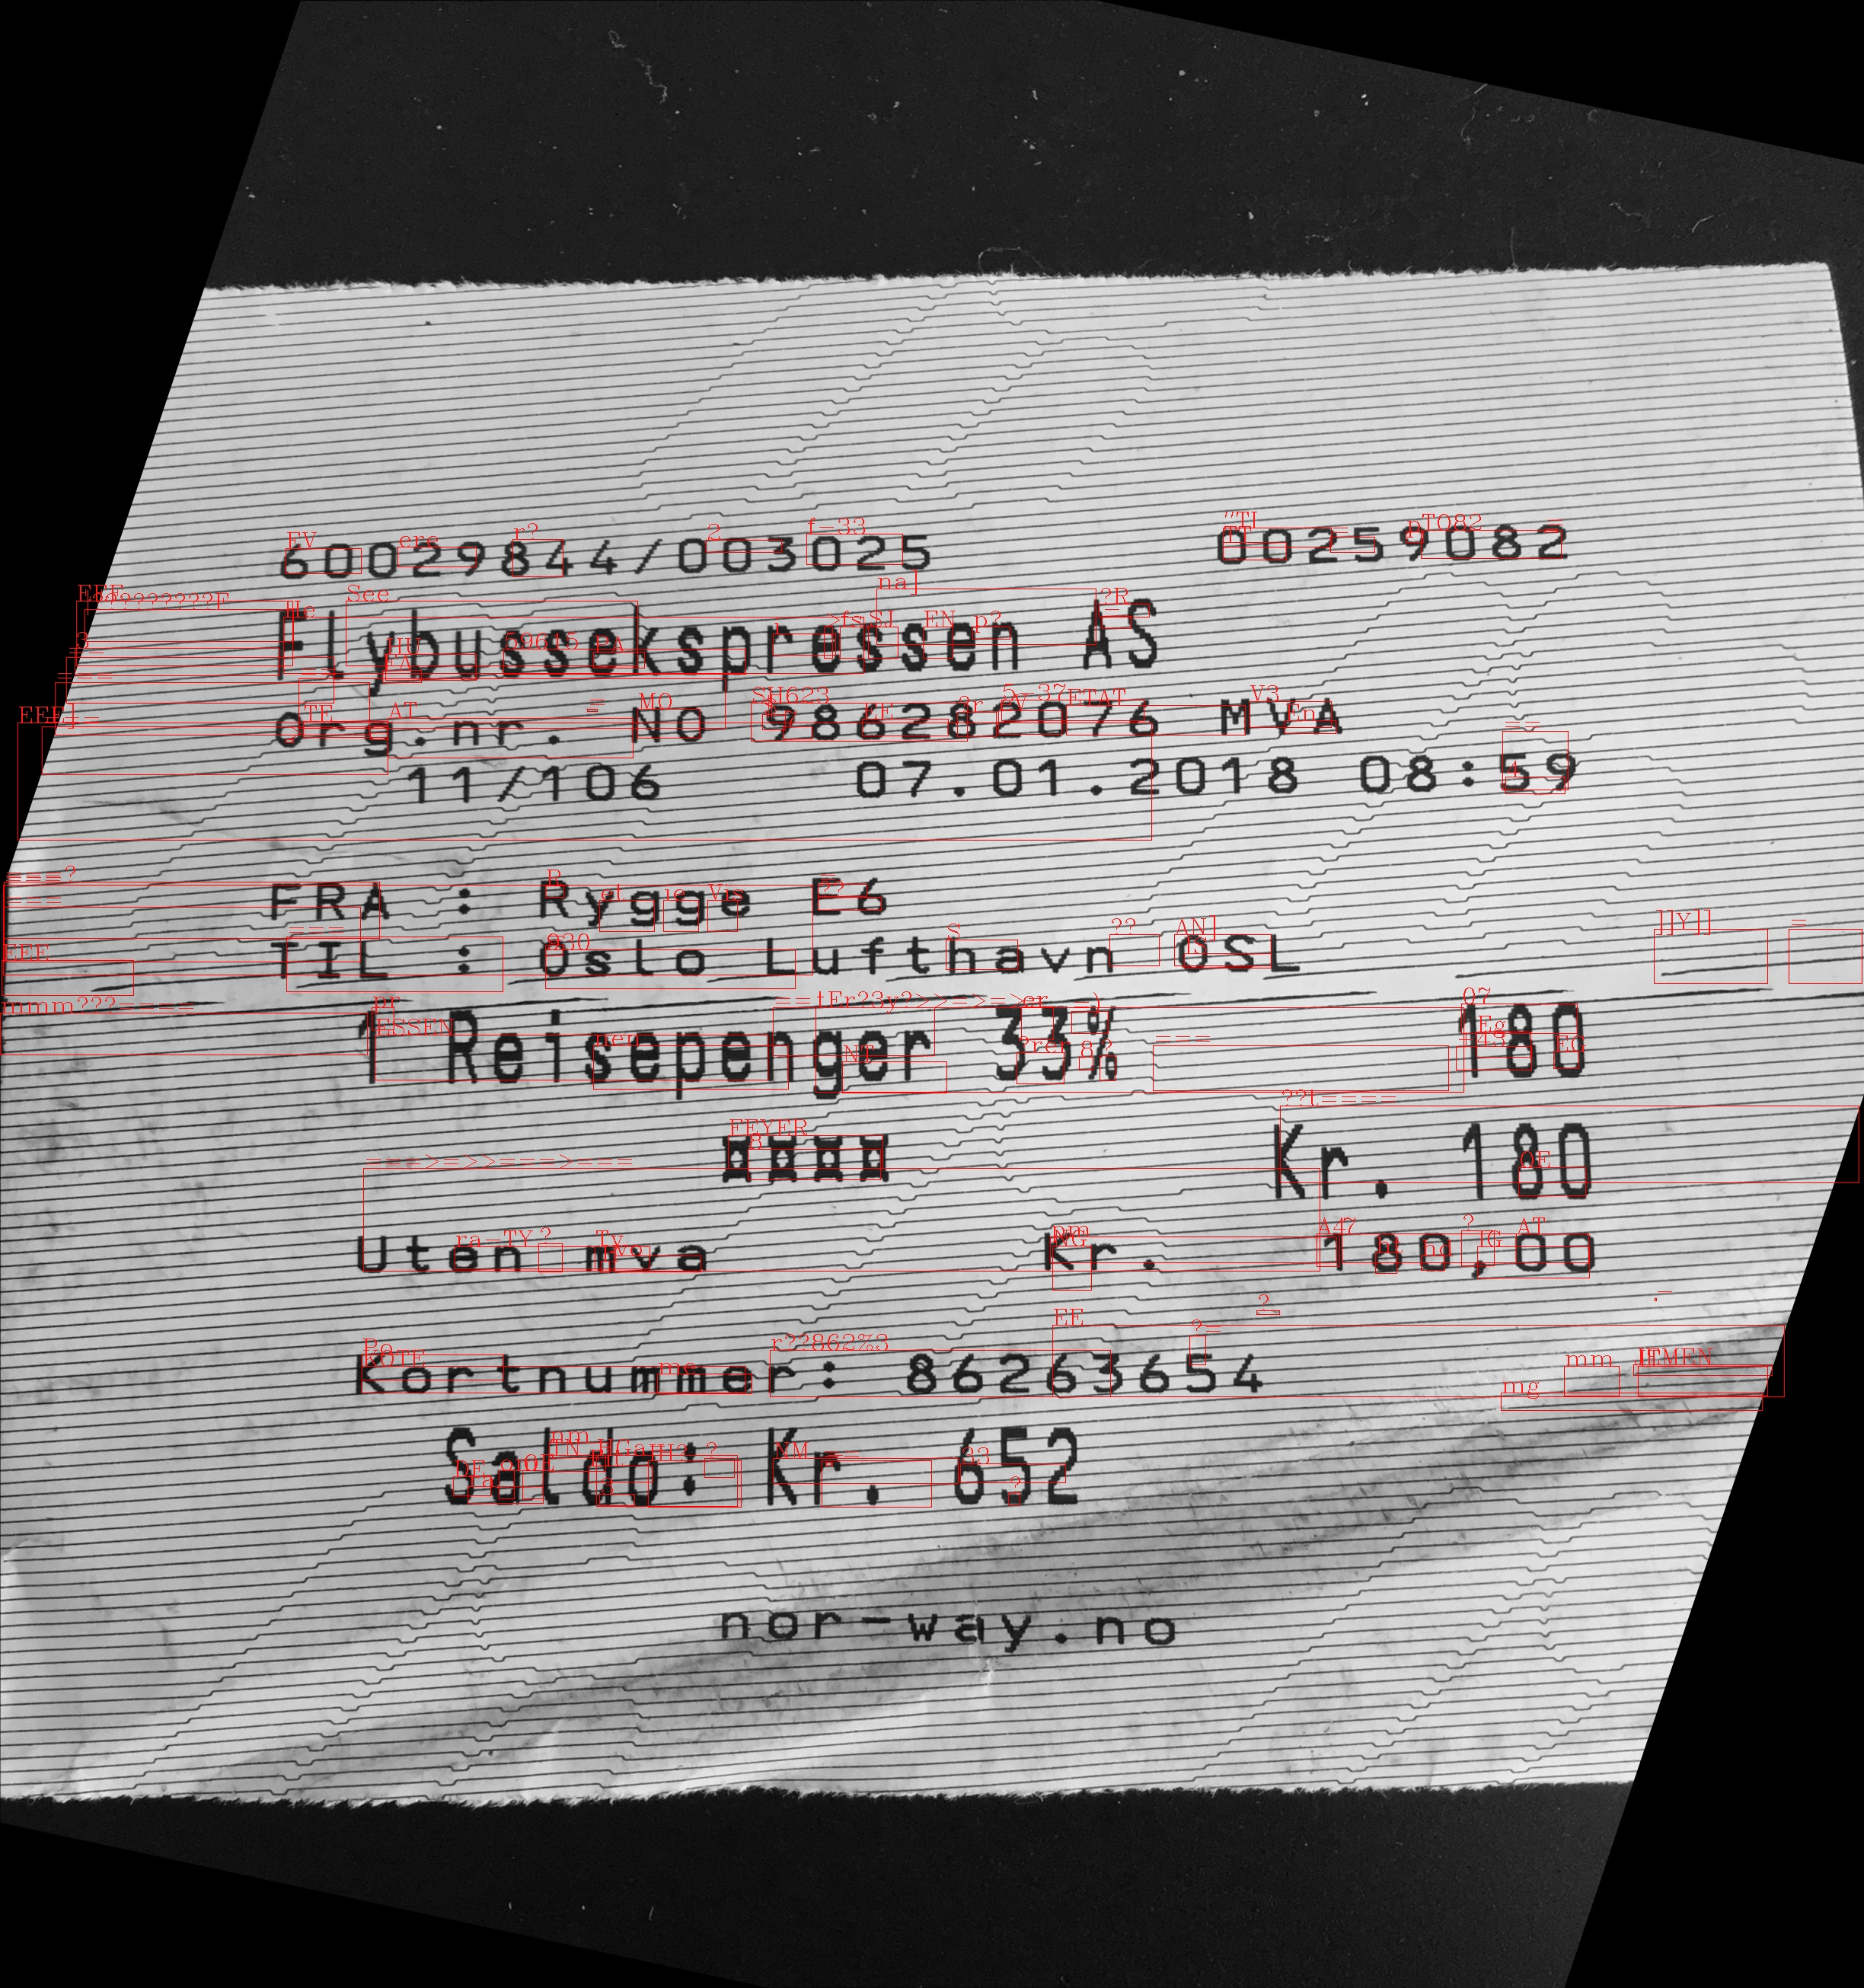
\includegraphics[width=1\textwidth]{Images/resultflybuss}}
    \caption{Extracted text in red, appearing over the place it has been extracted from}
    \label{fig:resultflybuss}
\end{figure}

Looking at the extracted text in figure~\ref{fig:resultflybuss}, it is apparent that the OCR did not
extract much useful information from the image.
Text is being found incorrectly along the edge of the receipt and in empty spaces in the receipt.
This is a recurring problem for receipts of this type, and will be discussed more in chapter 6.

\section{NER results}\label{sec:ner-results}
The text output from our OCR module is passed to our Spacy NER module for price extraction.
We were not able to extract any price information from Spacy's NER\@.

\section{Overall results}\label{sec:overall-results}

